\section{Introduction}\label{introduction} %Oscar and David
As th



\section{Related Work}\label{related_work} %David
On the current state of the Web, huge amount of data are exposed following the principles of Linked Data. We describe the main contributions on this topic, and also the relevance of the ones made in querying data on the web and the current solutions on planning transport routes using semantics.
%about linked data fragments and route planning with semantics
\subsection{Linked Data}
%what is linked data and its benefits
One of the most well-known alternatives to publish data on the Web is Linked Data \cite{bizer2009linked}. Linked Data allows to identify in an unique way resources on the Web using identifiers, or HTTP URIs. It is a method to distribute and scale data over large organizations such as the Web. When looking up this identifier by using the HTTP protocol or using a Web browser, a definition must be returned, including links towards potential other interesting resources, a practice called \textit{dereferencing}. The triple format to be used in combination with URIs is standardized within RDF. The URIs used for these triples already existed in other data sources, and we thus favored using the same identifiers. It is up to a data publisher to make a choice on which data sources can provide the identifiers for a certain type of entities. 

There are multiple benefits of exposing the data on the Web as Linked data: i) the data is linked to related data so the information can be combined across different interfaces, ii) the data is queryable using the query language for RDF, SPARQL \cite{prud2006sparql}, or other approaches like API-Rest interfaces \cite{world2014json} or \cite{lanthaler2013creating} iii) the data is represented following a reference model, so the interoperability between different data sources is at the semantic level.

In transport domain


\subsection{Querying data on the Web}

\subsection{Route planners}



\begin{figure}[h]
	\centering
	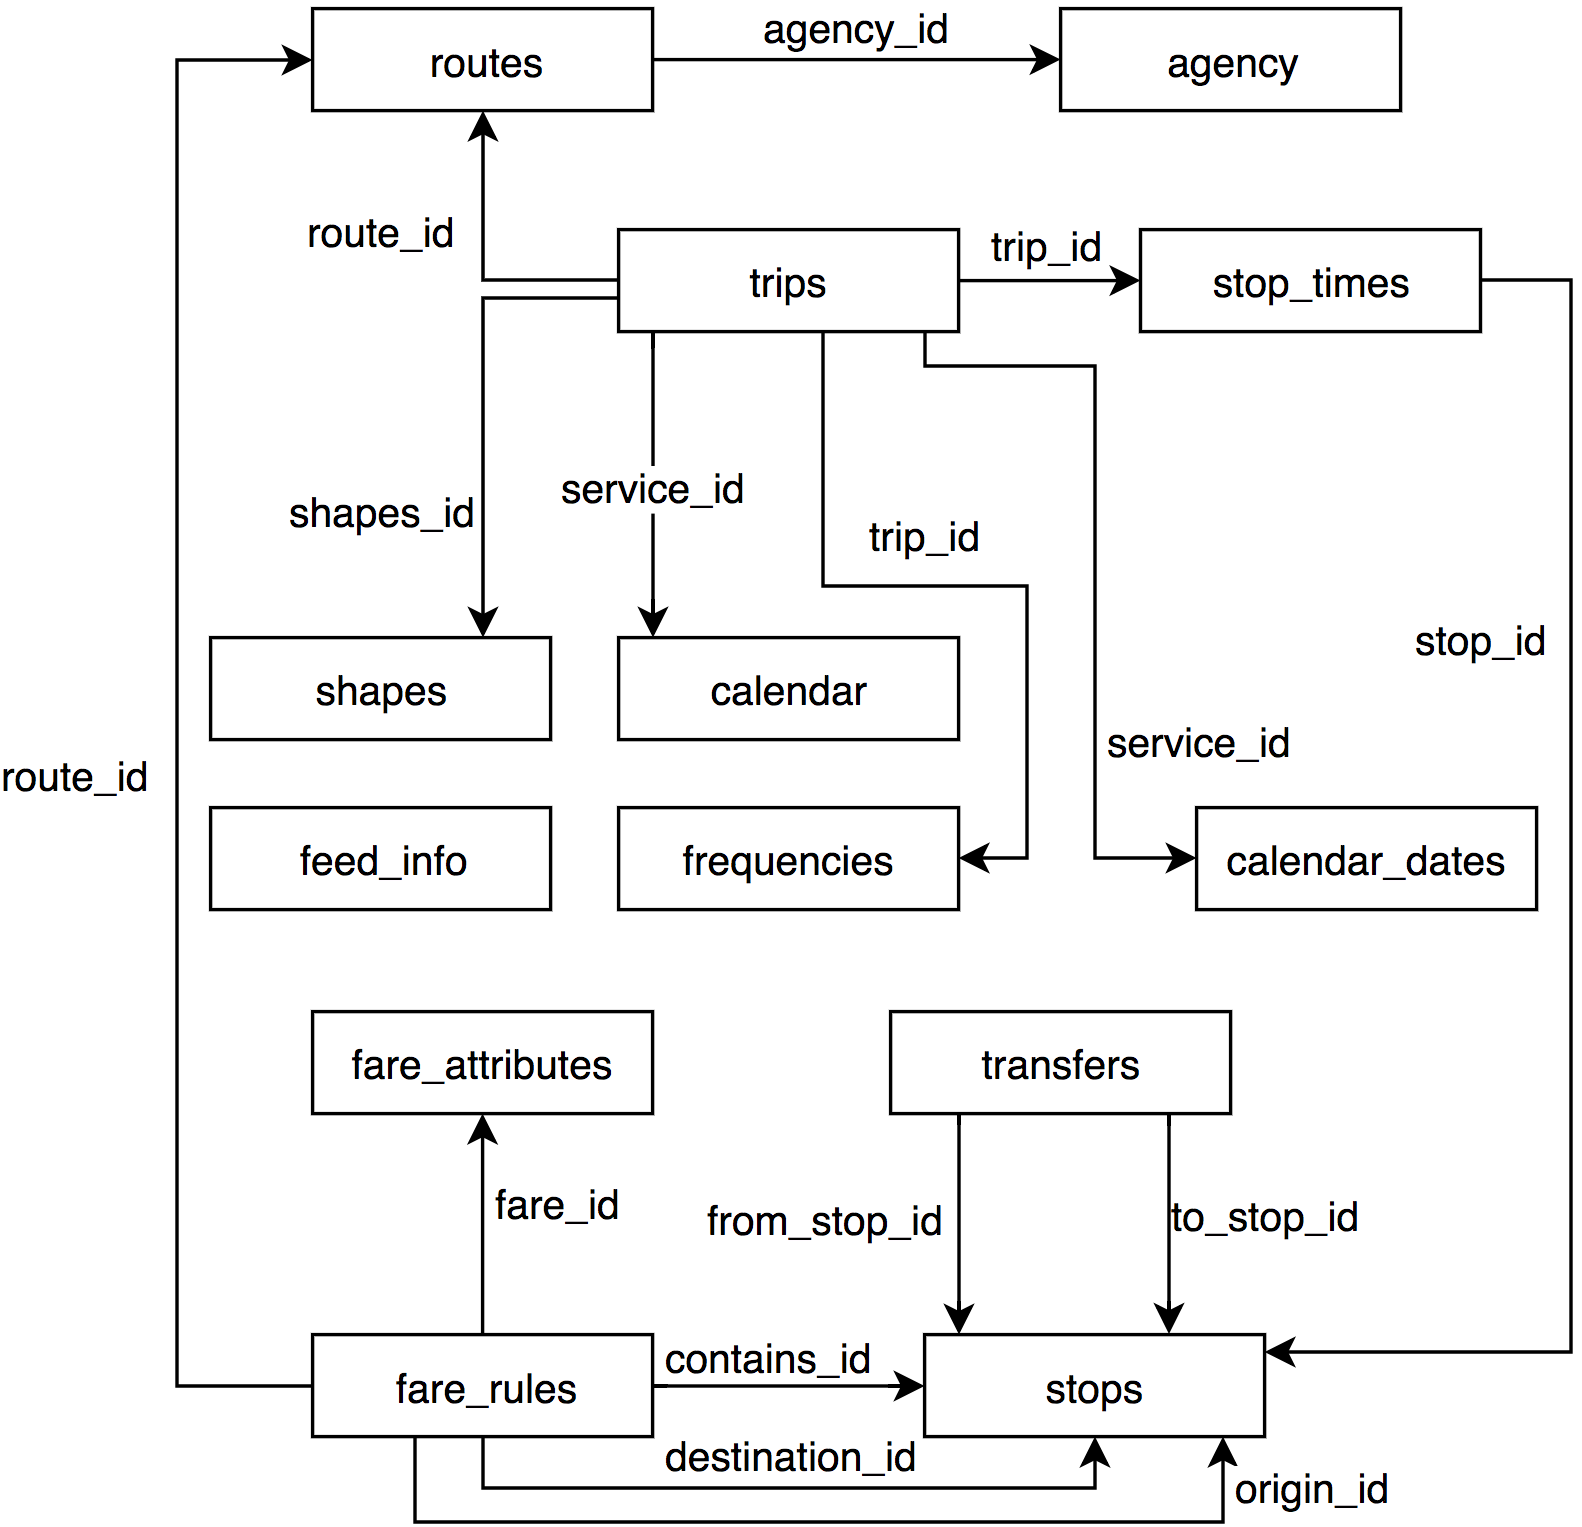
\includegraphics[width=1.0\linewidth]{images/gtfsmodel.png}
	\caption{Underlying GTFS schema}
	\label{fig:gtfs}
\end{figure}

\section{Linked Connections}

\subsection{Linked Connections Server}

\subsection{The Memento Protocol}

\subsection{TransportDCAT-AP}

\section{Evaluation Design}

\section{Results}

\section{Discussion}

\section{Conclusions and Future work}

\begin{acks}

\end{acks}